% TASK58_DRAFT_STUB
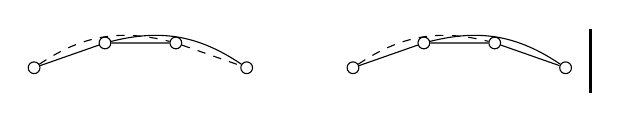
\begin{tikzpicture}[
  x=0.9cm,
  y=0.9cm,
  vertex/.style={circle,draw=black,fill=white,inner sep=1.5pt},
  positive/.style={draw=black,solid},
  negative/.style={draw=black,dashed}
]
  \node[vertex] (a0) at (0,0) {};
  \node[vertex] (a1) at (1,0.35) {};
  \node[vertex] (a2) at (2,0.35) {};
  \node[vertex] (a3) at (3,0) {};
  \draw[positive] (a0)--(a1)--(a2);
  \draw[negative] (a2)--(a3);
  \draw[negative,bend left=24] (a0) to (a2);
  \draw[positive,bend left=24] (a1) to (a3);

  \node[vertex] (b0) at (4.5,0) {};
  \node[vertex] (b1) at (5.5,0.35) {};
  \node[vertex] (b2) at (6.5,0.35) {};
  \node[vertex] (b3) at (7.5,0) {};
  \draw[positive] (b0)--(b1)--(b2)--(b3);
  \draw[negative,bend left=24] (b0) to (b2);
  \draw[positive,bend left=24] (b1) to (b3);
  \draw[black,line width=0.8pt] (7.85,-0.35)--(7.85,0.55);
\end{tikzpicture}
